\section{Sensitivity to Deterministic Parameter Choice}
\label{sec:AngleResults}

At this point in the $\Omega$-method characterization,
it has been shown how the $\Omega$-methods
behave in problems with differing geometries and materials.
However, each of the problems presented in Section \ref{sec:CharResults}
was run with the same deterministic calculation
parameters. While the angular flux may have differed in these problems due to
differences in the way the problems were constructed, it did not
vary due to deterministic
solver choices. Some deterministic solver choices will change the angular
fluxes used to calculate the $\Omega$-flux. Consequently, this may affect the
behavior of the $\Omega$-methods. This section will
explore the effects of deterministic solver
choices on the $\Omega$-method's performance.

Section \ref{sec:CharResults} showed that the $\Omega$-methods have a strong
weakness to ``thin'' materials, as CADIS and FW-CADIS do. Recall that a
``thin'' material is characterized by a low density, and thus a low macroscopic
cross section, or interaction
probability. In a pure streaming problem, the particle flux will decrease by a
factor of $r^2$ from the source and never interact.
In a thin material, a particle may stream
several centimeters before interacting. As a result, the
importance of a particle, which is related to the adjoint- or omega-flux,
may vary several orders of magnitude over a mean free
path of travel distance. At a collision, the particle then requires
several orders of
magnitude of sampling events.

The $\Omega$-method's weakness to ``thin'' materials was confirmed by
running the steel beam problem with air and concrete in the geometric location
of the steel beam. In
the ``thin'' material air version, CADIS-$\Omega$ performed poorer than CADIS.
This was a strong contrast to the same geometric configuration with a steel
beam, where CADIS-$\Omega$ outperformed CADIS.
The success of CADIS-$\Omega$ in this problem also showed that
the incorporation of the $\Omega$-flux into a problem with materials with
very different moderating properties but both with high probabilities of
interaction, improves the performance of the $\Omega$-methods beyond CADIS or
the nonbiased analog.

Due to CADIS-$\Omega$'s superior performance to CADIS
in the problem with a steel beam in concrete, this is the problem that will be
used to characterize CADIS-$\Omega$'s sensitivity to deterministic
parameter choice.
In this section, the effect of deterministic solver choices on the
performance of the $\Omega$ methods will be investigated. In particular, we are
interested in how parameters that influence the angular flux will affect the
performance of the $\Omega$-methods. By using the same problem
with differing solver options, the effect of solver options can be isolated from
the material and geometric effects. By doing so, we seek to determine how
resilient the $\Omega$-methods may be to using low-fidelity solver options, how
different the sensitivity of the $\Omega$-methods are to solution quality when
compared to CADIS, and how varying angular parameters may speed up or slow down
the time to a desired solution. By quantifying these effects, we can determine
the best parameter selection for the $\Omega$-methods for this type of problem.

\subsection{Parametric Study Description}
\label{subsec:parstudy}

The angle sensitivity parametric study will cover the subset of computational parameters
that are most likely to influence the $\Omega$ method's solution. Because the
$\Omega$-flux is calculated from an angular integration of the forward and adjoint
flux, calculation parameters that are most likely to influence the angular flux
solution are the variables that will be perturbed.
The two parameters that will be studied
are the quadrature order and the P$_N$ order.

The quadrature used in a deterministic solver is used do discretize the
problem in angle. Quadrature options are split into two separate selections: the
quadrature set or type, and the quadrature order. Because the $\Omega$-methods
require rotational symmetry, only quadrature sets that have rotational
symmetry (generally these are triangular quadrature sets)
can be used with the $\Omega$-methods. In ADVANTG/Denovo, the triangular
quadrature sets are: linear-discontinuous finite element, level-symmetric, and
quadruple range. As discussed previously, quadruple range is selected as the
ADVANTG default because it has good properties and guarantees positivity in the
flux. Different quadrature sets have separate
properties and are a realm of study unto their own. Thus, we will vary only
quadrature order and not quadrature type in this sensitivity study.

Quadrature orders specify
how fine of a resolution the quadrature set will be. As quadrature order
increases, the angular discretization becomes finer, and the
size of the angular flux matrices increases. The $\Omega$ methods use angular
flux values that are written to a file after a Denovo transport solve, which are
then read into memory to compute the $\Omega$-flux. We expect to
observe much slower deterministic recorded times in T$_{det}$--and, by
extension, T$_{hybrid}$--for high quadrature orders
because of the I/O demand to read and write the angular flux values. This I/O
demand will not be as extreme for standard CADIS, as the angular flux values are
not written in that case.
Recall that the ADVANTG
default quadrature order is 10. The quadrature orders used for the sensitivity
study aimed to choose orders surrounding this value. This resulted in quadrature
orders 5, 7, 10, 12, 15, 17, and 20 being chosen for variations in this
parameter.

The P$_N$ order determines the fidelity of the scattering expansion. The
availability of P$_N$ orders is dependent on the cross section dataset that is
being used. For the
27G19N cross section library, the P$_N$ order extends to 5. As a result,
P$_N$ orders of 1, 3, and 5 are chosen for variations in this parameter.

While the P$_N$ order
does affect angular information in the problem, it will not change the size of
the angular flux matrices. As a result, deterministic runtimes between
differing P$_N$ orders
may vary, but not as significantly as they will in differing quadrature orders
due to the lack of change in I/O requirements as P$_N$ order changes.

Other deterministic parameters may influence the variance reduction parameters
calculated by the $\Omega$ methods.
The spatial discretization, while not a primary factor influencing
the angular flux, still may affect the $\Omega$-methods' performance.
A finer energy group structure may also influence the $\Omega$-method solution.
Finer energy groups will more effectively reflect resonance regions in
scattering and absorption. Scattering effects in certain energy regions will
have angular dependence and, thus, may have a stronger effect on the angular flux
than a coarser energy discretization. Because these particular solution effects
do not directly influence the angular flux and angular effects will be difficult
to isolate, they will not be included
in the angular sensitivity parametric study.

% Add to conclusion future work.
%However, a study extending to include the
%energy group structure, the spatial discretization, and the quadrature type
%certainly could be an area of future work.

Several factors in the deterministic calculation should not have a strong effect
on the angular flux distribution. These include the spatial solver, the
convergence criteria for the solvers, and the within group solver types.
Because these factors should not influence the angular flux any more than any
other part of the solution, they will also not be included in this parametric study.

\subsection{Quadrature Order}
\label{subsec:quadorder}

The results that will be presented in the next two subsections will be similar
to those presented in Section \ref{sec:CharResults}. However, our goal is to see
how changing deterministic parameter type affects the results in the tally
region. With this in mind, the presentation of the results may be adjusted to
more effectively show the effect each parameter has on influencing the Monte
Carlo transport.

Table \ref{tab:quad_foms} contains the FOM results for each of the quadrature
orders run in the parametric study. The results are grouped by FOMs calculated
with the same relative error. The first three sections of the table
pertain to different FOM values, and the last section of the table shows timing
results for the standard Monte Carlo (T$_{MC}$) and the total walltime
(T$_{hybrid}$) for the calculation.

In the tally average relative error subsection of Table \ref{tab:quad_foms},
two strong
dips in the FOM appear in the CADIS results at S$_N$ orders 5 and 10,
and a dip in the CADIS-$\Omega$ FOMs
occur at S$_N$ order 12. These dips are much larger relatively than in the maximum or
minimum relative error subsections of the table. This indicates that for these
particular quadrature orders, fewer particles contribute to the
detector response across all groups. We can also see in the CADIS-$\Omega$
results that
quadrature orders 10, 15 and 17 all have a similar FOM for the tally average
relative error using the Monte Carlo runtime. However, the FOMs for the same
quadratures do not decrease more significantly when using T$_{hybrid}$ to calculate the
FOM, as suggested in Section \ref{subsec:parstudy}. This suggests that the
increased deterministic runtime for I/O is offset consistently by the change in
the FOM between quadrature orders for CADIS-$\Omega$.

In this subsection of the table it is also notable that the oscillations between
maximum and minimum FOM values is much larger for CADIS-$\Omega$ than for CADIS.
For low quadrature orders, CADIS-$\Omega$ shows substantial improvement in the
FOM, while CADIS remains somewhat constant (this is omitting the major dips in FOM
values noted in the previous paragraph). At higher quadrature orders, however,
CADIS-$\Omega$'s performance is inverted and decreases with increasing
quadrature order. CADIS, however, remains fairly constant in FOM for S$_N$
orders 12 and above. Both methods far outperform the nonbiased analog Monte
Carlo run.

The maximum relative error portion of the table also has several notable
datapoints. For CADIS, the dips in FOM are still visible for S$_N$ orders 5 and
10, but quadrature order 7 does not achieve the same high FOM as quadrature
orders 12 and above as it does in the tally average subsection of the table. If
the maximum relative error convergence is the limiting factor for the user,
it appears that using any quadrature order above 10 is a good choice for CADIS.
CADIS-$\Omega$, conversely, has more varied results. No observable trend exists
in the FOM with increasing quadrature order for CADIS-$\Omega$. A dip
in the FOM occurs at quadrature order 12, as it did in the tally average
subsection of the table. This dip, like CADIS' dips, is not as significant as
the dip in the tally average FOMs. Generally, CADIS has higher FOMs when using
the maximum relative error as a success metric. In fact, the only quadrature order where
CADIS-$\Omega$'s FOM is larger than CADIS' is at quadrature order 10.


\begin{table}[h!]
  \centering
  \begin{tabular}{lc|ccccc}
\toprule
{} & {} & \multicolumn{2}{c}{CADIS}  & \multicolumn{2}{c}{CADIS-$\Omega$}  & analog \\
{} &  S$_N$ order &     MC  &   MC$_{hybrid}$ & MC & MC$_{hybrid}$ &  MC \\
\midrule
\multirow{7}{*}{tally avg} &  S$_N$ 5 &        683 &       677 &   1.81e+03 &
1.79e+03 &  \multirow{7}{*}{1.39} \\
      {}     &  S$_N$ 7 &   2.55e+03 &  2.53e+03 &   2.46e+03 &     2.45e+03 &    {}   \\
      {}     & S$_N$ 10 &        669 &       659 &   2.96e+03 &     2.93e+03 &    {}   \\
      {}     & S$_N$ 12 &   2.46e+03 &  2.41e+03 &        187 &          183 &    {}   \\
      {}     & S$_N$ 15 &   2.48e+03 &  2.42e+03 &   2.98e+03 &     2.92e+03 &    {}   \\
      {}     & S$_N$ 17 &   2.47e+03 &  2.39e+03 &   2.96e+03 &     2.88e+03 &    {}   \\
      {}     & S$_N$ 20 &   2.46e+03 &  2.35e+03 &   1.89e+03 &     1.81e+03 &    {}   \\
\midrule
\multirow{7}{*}{max RE}  &  S$_N$ 5 &       4.89 &      4.85 &       2.86 &
2.84 &  \multirow{7}{*}{0.0448} \\
      {}     &  S$_N$ 7 &       7.71 &      7.64 &       4.35 &         4.32 &    {}   \\
      {}     & S$_N$ 10 &       3.74 &      3.69 &       6.71 &         6.64 &    {}   \\
      {}     & S$_N$ 12 &       14.3 &      14.1 &      0.764 &        0.748 &    {}   \\
      {}     & S$_N$ 15 &       14.7 &      14.3 &       3.87 &         3.79 &    {}   \\
      {}     & S$_N$ 17 &       14.8 &      14.4 &       7.98 &         7.78 &    {}   \\
      {}     & S$_N$ 20 &       14.1 &      13.5 &       6.09 &         5.85 &    {}   \\
\midrule
\multirow{7}{*}{min RE}  &  S$_N$ 5 &   1.14e+03 &  1.13e+03 &   1.09e+03 &     1.09e+03 &      -- \\
      {}     &  S$_N$ 7 &   1.37e+03 &  1.36e+03 &   1.26e+03 &     1.25e+03 &      -- \\
      {}     & S$_N$ 10 &   1.43e+03 &  1.41e+03 &   1.32e+03 &      1.3e+03 &      -- \\
      {}     & S$_N$ 12 &   1.46e+03 &  1.43e+03 &   1.33e+03 &      1.3e+03 &      -- \\
      {}     & S$_N$ 15 &   1.47e+03 &  1.43e+03 &   1.32e+03 &      1.3e+03 &      -- \\
      {}     & S$_N$ 17 &   1.46e+03 &  1.42e+03 &   1.31e+03 &     1.28e+03 &      -- \\
      {}     & S$_N$ 20 &   1.46e+03 &  1.39e+03 &   1.31e+03 &     1.26e+03 &      -- \\
\midrule
\multirow{7}{*}{Time (mins)}  &  S$_N$ 5 &        302 &       305 &   1.13e+03 &
1.14e+03 &    \multirow{7}{*}{22.3} \\
      {}     &  S$_N$ 7 &        324 &       327 &   1.62e+03 &     1.63e+03 &    {}   \\
      {}     & S$_N$ 10 &        414 &       420 &   2.11e+03 &     2.14e+03 &    {}   \\
      {}     & S$_N$ 12 &        406 &       414 &   2.09e+03 &     2.14e+03 &    {}   \\
      {}     & S$_N$ 15 &        404 &       413 &    2.1e+03 &     2.14e+03 &    {}   \\
      {}     & S$_N$ 17 &        405 &       418 &   2.11e+03 &     2.17e+03 &    {}   \\
      {}     & S$_N$ 20 &        406 &       425 &   2.12e+03 &     2.21e+03 &    {}   \\
\bottomrule
\end{tabular}

  \caption[Figure of Merit results for steel beam embedded in concrete, with
  variations in quadrature order.]{Figure of Merit results for steel beam embedded in concrete, with
  variations in quadrature order. Subdivisions of the table indicate
calculations of the FOM using different relative errors. The analog case has a
single value for each relative error as it is not dependent on changes in
deterministic calculation parameters.}
  \label{tab:quad_foms}
\end{table}

In the minimum relative error subsection of Table \ref{tab:quad_foms}
the CADIS and CADIS-$\Omega$ FOM behavior is
much more well-behaved than it is for the preceding two subsections of the
table. There are no dips in the FOM value for either method,
so the lowest relative error will
consistently get better with increasing quadrature order. A slight shift
to a $<1\%$ lower FOM
occurs for quadrature orders 17 and 20, which indicates that increasing
quadrature fidelity does not help improve the FOM past S$_N$ order 15. Similar
behavior is observable for CADIS-$\Omega$ in the minimum relative error
subsection of the table. CADIS-$\Omega$ has a consistently lower-valued FOM
between ~5\%-10\% for all quadrature orders when compared to CADIS.
A turnover occurs in the CADIS-$\Omega$
FOMs at a lower quadrature order, meaning that CADIS-$\Omega$ does not benefit
from increasing S$_N$ order as much as CADIS using this FOM as a metric.
However, beyond quadrature order 15 neither method sees a benefit in the FOM by
increasing the quadrature order.

The timing results in the last section of the table show how much longer it
takes CADIS-$\Omega$ to transport the standard Monte Carlo than CADIS. This was
also noted in Section \ref{subsec:resultbeam}. In the
introduction to this section, it was predicted that the I/O demands for
CADIS-$\Omega$ would impact the MC$_{hybrid}$ FOMs as quadrature order
increases. However, because the CADIS-$\Omega$ Monte Carlo times are already so
much longer than CADIS', this impact is not as significant as expected. Further,
the increase in deterministic runtime seems to change similarly to the increase
in Monte Carlo runtime as the importance map changes. This explains why the FOMs
were not impacted so negatively in the previous sections of the table.

Let us use an illustrative example to compare the FOMs between CADIS and
CADIS-$\Omega$. Returning again to Table
\ref{tab:quad_foms}, at S$_N$ order 5 the non-MC runtime is three minutes for
CADIS, while it is around ten minutes for CADIS-$\Omega$. At S$_N$ order 20, the
CADIS non-MC runtime is 19 minutes; the CADIS-$\Omega$ time is 100 minutes. For
each of these cases, the non-MC runtime is about 4\% that of the Monte Carlo runtime.
Because this fractional time is fairly consistent between CADIS and
CADIS-$\Omega$, we do not see a strong impact on FOM$_{hybrid}$ from the
significantly longer non-MC runtimes in CADIS-$\Omega$.

Table \ref{tab:quad_foms} shows that for the FOM using the tally average relative error,
CADIS-$\Omega$ outperforms CADIS for most quadrature orders (with excpetions
being S$_N$ orders 7 and 12). For the majority of the quadrature orders,
CADIS-$\Omega$ gets more particles to the tally region than CADIS in the same
amount of time. By increasing
quadrature order, CADIS-$\Omega$ generally increases the number of particles to
the tally as a whole, while CADIS remains fairly constant. The table
also shows that by using either the maximum or minimum relative error to
calculate the FOM, CADIS generally outperforms CADIS-$\Omega$. However, while
both the maximum and minimum RE FOMs increase with increasing quadrature order
in CADIS, this is not the case for the tally average FOM. This could be
interpreted as that as the quadrature order increases, more particles reach the extreme
tally bins, but fewer particles end up in the tally overall. For CADIS-$\Omega$,
this behavior is not quite the same. Instead, a peak occurs in the tally
average FOMs at intermediate quadrature orders, and the minimum RE FOM decreases
with increasing quadrature order.

\begin{figure}[htb!]
  \centering
  \begin{subfigure}[t]{\textwidth}
    \centering
    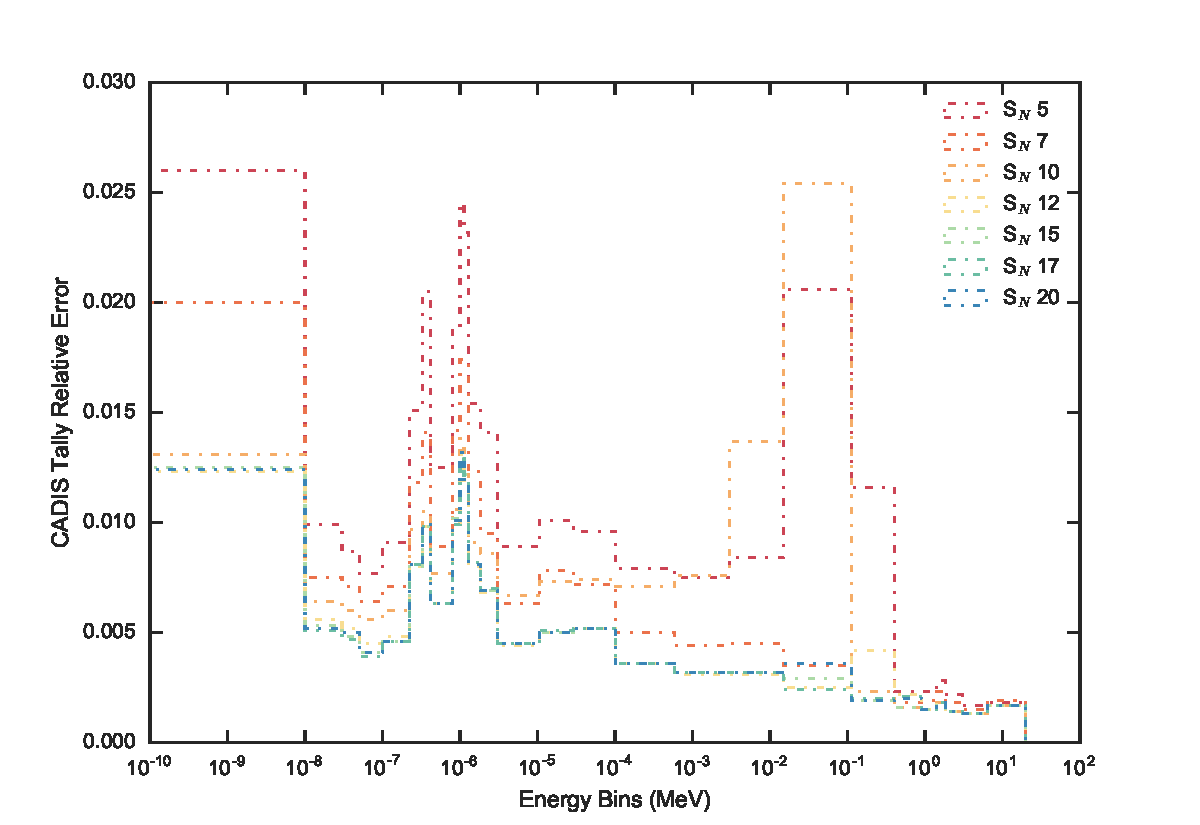
\includegraphics[width=\linewidth]{./chapters/characterization_probs/figures/angle/prob_1/err_quad_cadis.pdf}
    \caption{Relative errors of CADIS results for differing S$_N$ orders.}
    \label{fig:sn_cad_err}
  \end{subfigure}
\end{figure}
\begin{figure}[htb!]\ContinuedFloat
  \centering
  \begin{subfigure}[t]{\textwidth}
    \centering
    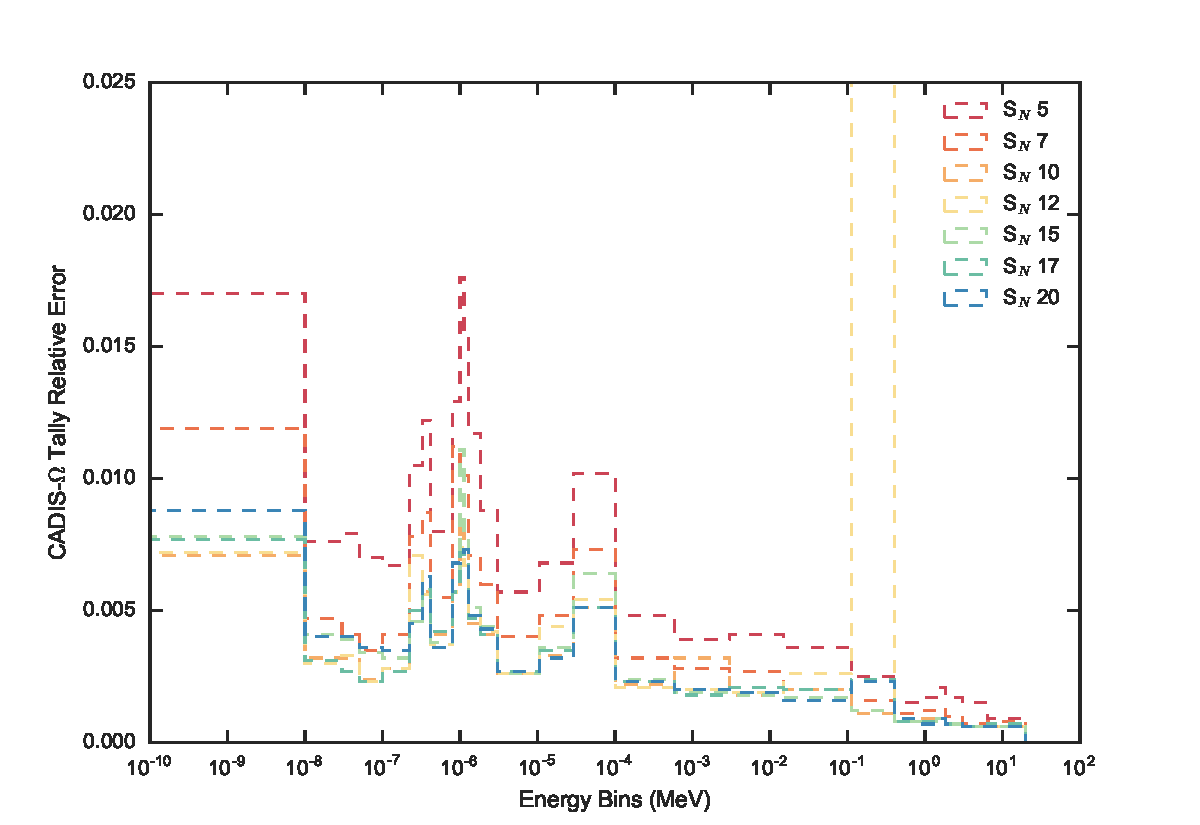
\includegraphics[width=\linewidth]{./chapters/characterization_probs/figures/angle/prob_1/err_quad_cadisangle.pdf}
    \caption{Relative errors of CADIS-$\Omega$ results for differing S$_N$
    orders.}
    \label{fig:sn_cadangle_err}
  \end{subfigure}
  \caption[Relative error results for CADIS and CADIS-$\Omega$ for different
  quadrature orders for the problem with a steel beam in concrete.]
  {Relative error results for CADIS (Figure \ref{fig:sn_cad_err})
  and CADIS-$\Omega$ (Figure \ref{fig:sn_cadangle_err}) for different
  quadrature orders for the problem with a steel beam in concrete.}
  \label{fig:sn_errs}
\end{figure}

In the Subsection \ref{sec:CharResults}, it was discussed that while the FOM
shows how quickly a tally may approach a desired value, it does not show how
effectively
each method transported particles to the tally location. Because the same
particle count was used in each variation of the steel beam problem in the angle
sensitivity study, the relative error results achieved by each method can reveal
how well each method transported the same number of starting particles.
The next several plots will present
this information.

Figures \ref{fig:sn_cad_err} and \ref{fig:sn_cadangle_err} show the relative
errors for all tally bins for each quadrature order run of the problem with the
steel beam in concrete for CADIS and CADIS-$\Omega$, respectively.
Unlike Table \ref{tab:quad_foms}, these plots show the
overall behavior of the tally results as a function of changing quadrature
order, so the behavior of non-extreme tally bins can also be observed. As noted
in the discussion accompanying Table \ref{tab:quad_foms}, these intermediate
are important in evaluating the tally average relative error.

Figure \ref{fig:sn_cad_err} plots the tally relative error results for each of
the CADIS runs, binned by energy. The warmer colored red and orange lines show
the low quadrature order results, while the cooler colored lines correspond to
higher quadrature results. For all of the energy bins below $10^{-4}$ MeV, a
reduction in the relative error with increasing quadrature order can be
observed. For quadrature orders S$_N$ 12 and above, the relative error does not
show as much of an improvement in the relative error. Between $10^{-4}$ and
$10^{0}$ MeV, large spikes in the relative error for quadrature orders 5 and 10
exist, explaining the poor behavior of the tally average RE FOM and tally
maximum RE FOM for CADIS.
Quadrature order 7 has relative errors much closer to quadrature orders
12 and above. Because these relative error spikes span so many bins, they affect
the overall tally convergence, and, by extension, the tally average FOM. At very
high energies ($> 10^{0}$ MeV), there is very little improvement in the relative
error with increasing quadrature order.

Figure \ref{fig:sn_cadangle_err} shows the relative error results for
CADIS-$\Omega$. A number of interesting features exist in
this figure that are not reflected in Figure \ref{fig:sn_cad_err}. For example,
in the lowest energy region a decrease in the relative error is seen up to S$_N$
10, but then the relative error increases for higher S$_N$ orders. In the wider
energy bins between
$10^{-6}$ and $10^{-1}$ MeV, quadrature orders 10 and above all achieve a
similar relative error. This is not true in narrow energy bins, where higher
quadrature orders do tend to have a lower relative error. Moving to higher
energies, we can observe a significant spike in the relative error between
$10^{-1}$ to $10^{0}$ MeV for S$_N$ order 12. Although this spike does not span
several energy bins like those seen in Figure \ref{fig:sn_cad_err}, it is very
high when compared to the other relative error bins. As a result, this single
tally bin throws off the tally average FOM results in addition to the tally
maximum RE FOM, as observed in Table
\ref{tab:quad_foms}. In energy bins above this spike, most quadrature orders
produce similar FOMs. The lowest valued energy bin is located in this high
energy region.

\begin{figure}[h!]
  \centering
  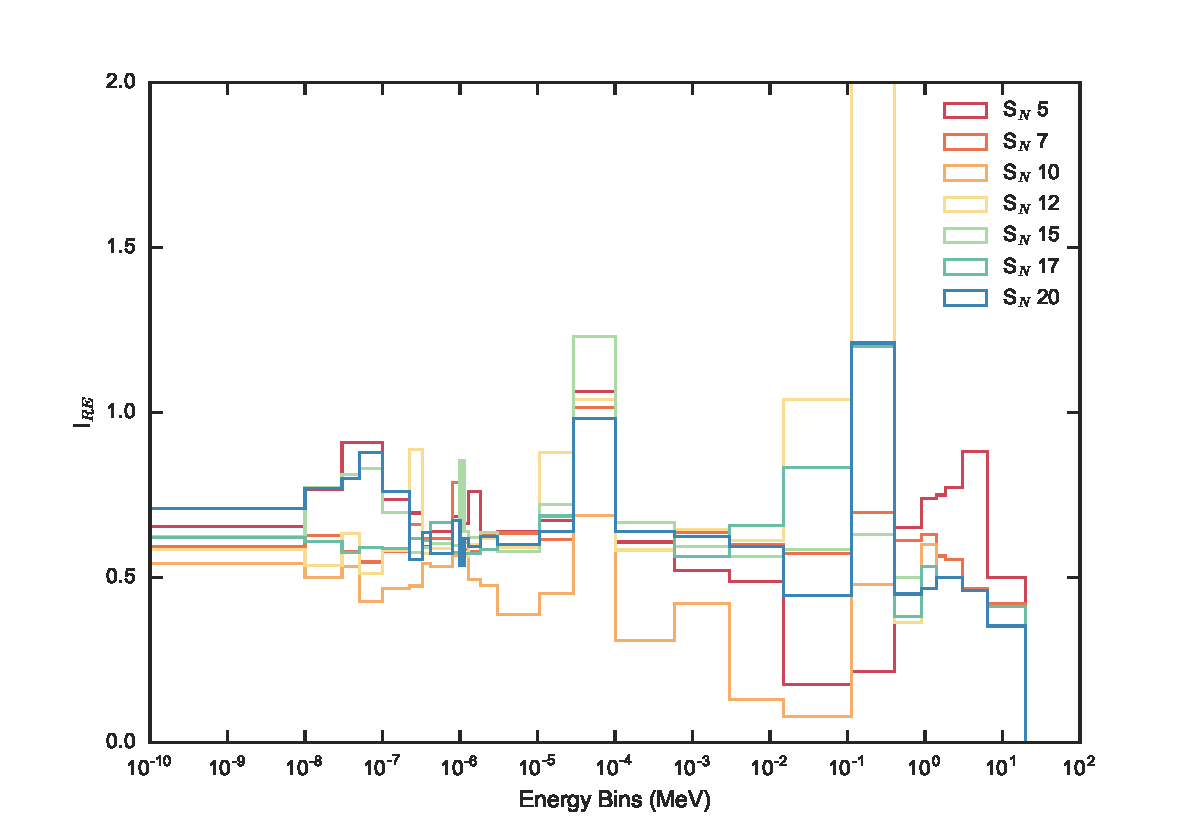
\includegraphics[height=10cm]{./chapters/characterization_probs/figures/angle/prob_1/compare_err_quad.pdf}
  \caption[Relative error improvement factor (Eq. \eqref{eq:I-RE}) between CADIS-$\Omega$ and
  CADIS as a function of quadrature order for steel beam embedded in concrete.]
  {Relative error ratio (Eq. \eqref{eq:I-RE}) between CADIS-$\Omega$ and
   CADIS as a function of quadrature order for the problem with
   a steel beam embedded in concrete.}
  \label{fig:prob_1_quad_I_RE}
\end{figure}

While Figure \ref{fig:sn_errs} shows the how the relative errors of the tally
change with different quadrature orders, we have no indication of how CADIS and
CADIS-$\Omega$ change in comparison to one another. Figure
\ref{fig:prob_1_quad_I_RE} shows the relative error improvement factor for each
quadrature order. A value below unity indicates that CADIS-$\Omega$ achieved a
better relative error than CADIS for that bin and quadrature order. In this
figure we can clearly see the effect that the problematic energy bins in each
method have on the improvement factor. In CADIS we observed that bins in the
$10^{-3}$ to $10^{-1}$ were problematic for quadrature order 10; this is
reflected in the very low value of I$_{RE}$ for that energy range and quadrature
order, as shown in by the orange line reaching the lowest values of I$_RE$.
Conversely, we observed that CADIS-$\Omega$ had a very problematic energy
bin between $10^{-1}$ and $10^{0}$ at quadrature order 12. The value of this
I$_{RE}$ is far above the y-limit of Figure \ref{fig:sn_errs}, illustrated with
the yellow line.

Figure \ref{fig:sn_errs} also shows that quadrature order 10 is generally the order
in which CADIS-$\Omega$ outperforms CADIS the most. For this quadrature error,
CADIS-$\Omega$ achieves the lowest error when compared to CADIS. The reasons for
this are twofold: first, it is one of the best performing quadrature sets for
CADIS-$\Omega$, which achieves its lowest relative errors in almost every energy
bin in this quadrature order; second, it is a very poorly performing quadrature
set for CADIS. This synergistic combination results in the best overall
quadrature order for CADIS-$\Omega$.

A region where quadrature order 10 is not the best quadrature order is
in energy regions above ~$10^{-1}$ MeV, whre the higher quadrature
orders--like 15, 17 and 20--outperform CADIS more.
In the low ($<10^{-5}$ MeV) and high ($>10^{0}$ MeV) energy
regions,
CADIS-$\Omega$ obtains lower relative errors than CADIS for all quadrature
orders. In intermediate energy regions, some spikes occur in regions that
indicate a lower relative error is achieved by CADIS. However, generally
CADIS-$\Omega$ achieves lower relative errors than CADIS for most energy bin and
most quadrature orders. Returning again to the
relative error figures of \ref{fig:sn_errs}, the spike in I$_{RE}$ between
$10^{-5}$ and $10^{-4}$
MeV is explained by a relatively low relative error achieved by CADIS, where in
CADIS-$\Omega$ a large spike in the relative error occurs. This is reflected in
the ratio for I$_RE$.

\begin{figure}[h!]
  \centering
  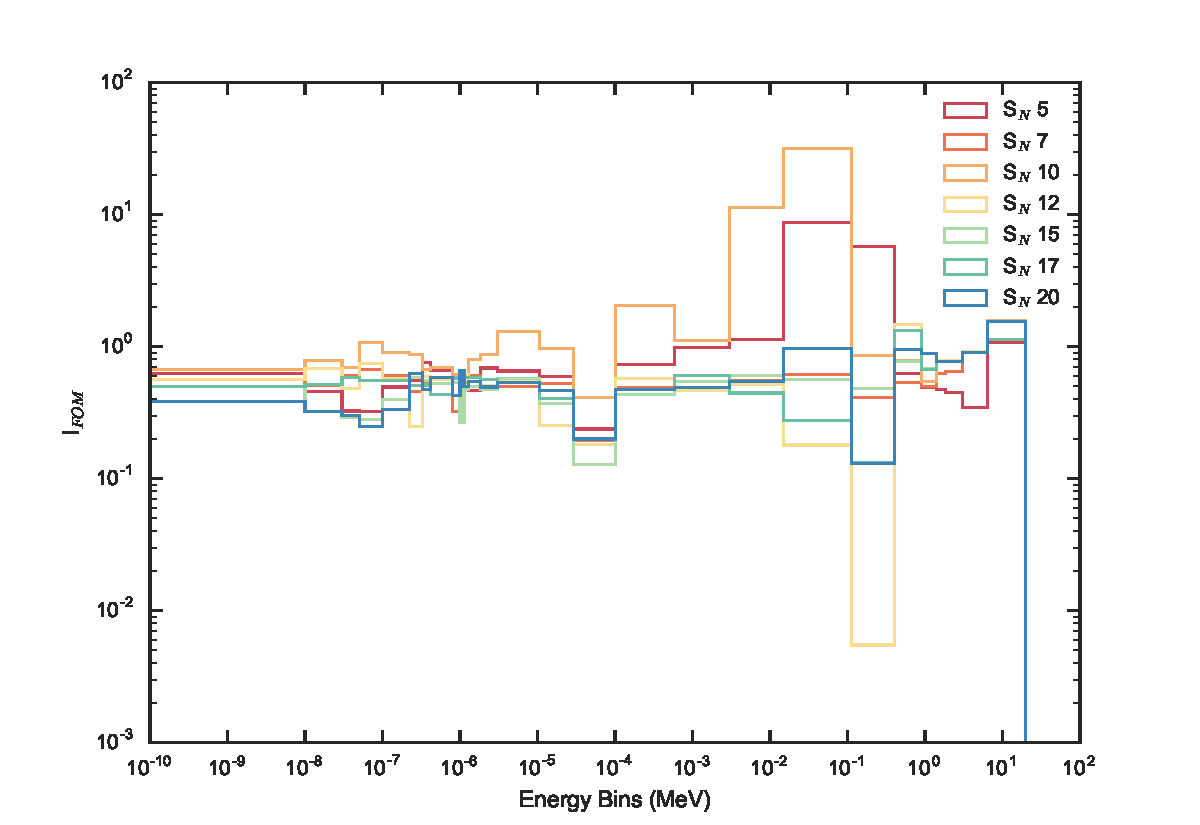
\includegraphics[height=10cm]{./chapters/characterization_probs/figures/angle/prob_1/compare_fom_quad.pdf}
  \caption[Figure of merit improvement factor  (Eq. \eqref{eq:I-FOM}) between CADIS-$\Omega$ and
  CADIS with changes in quadrature order for steel beam embedded in concrete.]
  {Figure of merit improvement factor  (Eq. \eqref{eq:I-FOM}) between CADIS-$\Omega$ and
   CADIS with changes in quadrature order for the problem with
   a steel beam embedded in concrete.}
  \label{fig:prob_1_quad_I_FOM}
\end{figure}

Figure \ref{fig:prob_1_quad_I_FOM} complements the results to Figure
\ref{fig:prob_1_quad_I_RE}. Here the FOM improvement factor is plotted rather
than the relative error improvement factor. Because a higher valued FOM is a
better result, values above $10^{0}$ indicate that CADIS-$\Omega$ outperformed
CADIS. On this plot it is quite clear that for higher energies, CADIS-$\Omega$
consistently outperforms CADIS more
in higher quadrature orders, as observed with I$_{RE}$.

Let us return again to the high and low-energy regions of the plot, as explored
with Figure \ref{fig:prob_1_quad_I_RE}. In this region it can be observed
that for low energies, generally I$_{FOM}$ decreases with increasing
S$_{N}$ order. This behavior reverses at high energies, where the ratio
increases with increasing quadrature order. This may be an effect of anisotropy
in each energy group, as the highest energy has the most anisotropy in the flux.
Recall from Section \ref{subsec:resultsbeam} that the anisotropy metric was much
higher at high energies than it was at low energies. It is possible that for
this more anisotropic energy group, increasing the quadrature order improves the
importance map in the $\Omega$ methods more, resulting in a better relative
error, and, consequently, a better FOM.
This would also explain the complementary behavior at low energies. Low
energies generally have more isotropic behavior, and increasing the quadrature
order would not help to improve anisotropy information in the importance map.
As a result, increasing quadrature order would not help the FOM at low energies.

Despite a higher relative FOM at high energies, in higher quadrature orders
CADIS-$\Omega$'s performance does not generally exceed CADIS'. For quadrature
order 20, CADIS-$\Omega$'s FOM is almost always lower than CADIS. On Figure
\ref{fig:prob_1_quad_I_FOM}, the cooler toned lines which correspond to higher
quadrature orders have lower values than the warmer toned lines.
For quadrature order 5,
the relative errors on Figure \ref{fig:prob_1_quad_I_RE} were bookended by
higher order quadratures at middle and low energies. This behavior is not the
same in Figure \ref{fig:prob_1_quad_I_FOM}, where the lowest quadrature order
has a higher relative FOM than any of the quadrature orders above 10. This means
that the time required to solve higher quadrature orders affects the FOM more
negatively than the quadrature order decreases the relative error (and
positively affects the FOM). It could also mean that the relative error
improvement changes more for CADIS than CADIS-$\Omega$ with increasing
quadrature order. As a result, the improvement factor at lower quadrature orders
is better for CADIS-$\Omega$ than at higher quadrature orders.

%[Show FOMs as a function of quad order for first problem] \\
%
%[Show interesting anisotropy plots for extreme-valued quad types.] \\
%
%[Show flux maps for each extreme-valued problem in region of interest.] \\
%
%[Describe results.] \\
%
%[Show FOMs as a function of quad order for second problem] \\
%
%[Show interesting anisotropy plots for extreme-valued quad types.] \\
%
%[Show flux maps for each extreme-valued problem in region of interest.] \\
%
%[Describe results.] \\

\subsection{Scattering (P$_N$) Order}
\label{subsec:pnorder}

Table \ref{tab:pn_foms} is much like that of Table \ref{tab:quad_foms}, but with
differing P$_N$ orders than quadrature orders. The table is split into four
regions, the first three corresponding to FOMs calculated with
different relative errors and the last corresponding to Monte Carlo and hybrid
runtimes for the problem. Each of the three first subsections of the table have
different trends with P$_N$ order, which will be described in the next several
paragraphs.

In the tally average relative error subsection of the table one can see that
CADIS has a dip in the FOM for P$_N$ order 3; both P$_N$ orders 1 and 5 are
higher overall. This effect is not seen in CADIS-$\Omega$, where a decrease in
the FOM is observed with increasing P$_N$ order. As a result, for
CADIS-$\Omega$, lower P$_N$ orders are sufficient for generating biasing
parameters, but for standard CADIS the highest P$_N$ order achieves the best
tally average FOM. Further, for every P$_N$ order, the tally average FOM is
higher for CADIS-$\Omega$ than CADIS.

As with Table \ref{tab:quad_foms}, a dip in CADIS' FOMs is also observable in the
maximum relative error subsection of the table. However, the dip observable at
P$_N$ order 3 also exists in the CADIS-$\Omega$ FOMs. If a user desires to have all
tally bins to be below a particular relative error, P$_N$ order 3 is the worst
option for both methods in this problem. For P$_N$ order 1 CADIS-$\Omega$ is the
better choice, and for P$_N$ order 5, CADIS is the better choice.

\begin{table}[h!]
  \centering
  \begin{tabular}{lc|ccccc}
\toprule
{} & {} & \multicolumn{2}{c}{CADIS}  & \multicolumn{2}{c}{CADIS-$\Omega$}  & analog \\
{} &  P$_N$ order &     MC  &   MC$_{hybrid}$ & MC & MC$_{hybrid}$ &  MC \\
\midrule
\multirow{3}{*}{tally avg} &  P$_N$ 1 &    1.76e+03 &  1.74e+03 &   2.99e+03 &
2.96e+03 &    \multirow{3}{*}{1.39} \\
     {}    &  P$_N$ 3 &         671 &       661 &   2.97e+03 &     2.94e+03 & {} \\
     {}    &  P$_N$ 5 &    2.21e+03 &  2.16e+03 &   2.45e+03 &     2.42e+03 & {}  \\
\midrule
\multirow{3}{*}{max RE} &  P$_N$ 1 &        7.19 &      7.09 &       8.06 &
7.98 &  \multirow{3}{*}{0.0448} \\
     {}    &  P$_N$ 3 &        3.75 &       3.7 &       6.74 &         6.66 & {} \\
     {}    &  P$_N$ 5 &        14.8 &      14.5 &       8.24 &         8.12 & {} \\
\midrule
\multirow{3}{*}{min RE} &  P$_N$ 1 &     1.5e+03 &  1.48e+03 &   1.33e+03 &     1.31e+03 &      -- \\
     {}    &  P$_N$ 3 &    1.43e+03 &  1.41e+03 &   1.32e+03 &     1.31e+03 &      -- \\
     {}    &  P$_N$ 5 &    1.24e+03 &  1.22e+03 &   1.57e+03 &     1.55e+03 &      -- \\
\midrule
\multirow{3}{*}{time (mins)} &  P$_N$ 1 &         394 &       399 &   2.09e+03 &
2.11e+03 &    \multirow{3}{*}{22.3} \\
     {}    &  P$_N$ 3 &         413 &       419 &    2.1e+03 &     2.13e+03 & {}  \\
     {}    &  P$_N$ 5 &         559 &       571 &   2.55e+03 &     2.59e+03 & {} \\
\bottomrule
\end{tabular}

  \caption[Figure of Merit results for steel beam embedded in concrete, with
  variations in P$_{N}$ order.]{Figure of Merit results for steel beam embedded in concrete, with
    variations in P$_{N}$ order. Subdivisions of the table indicate
calculations of the FOM using different relative errors. The analog case has a
single value for each relative error as it is not dependent on changes in
deterministic calculation parameters.}
  \label{tab:pn_foms}
\end{table}

Comparing the FOMs for CADIS and CADIS-$\Omega$ using the minimum relative
errors, some interesting trends are visible. In Table \ref{tab:quad_foms} we
observed that as quadrature order increased, the minimum relative error FOM
generally increased or stayed the same for both CADIS and
CADIS-$\Omega$. This is not the case in Table \ref{tab:pn_foms}. As P$_N$ order
increases, the minimum relative error FOM for CADIS decreases, but for
CADIS-$\Omega$ it increases. This means that increasing P$_N$ order does not
move more particles (and reduce the relative error) in the energy bin with the
lowest relative error in CADIS, but it does in CADIS-$\Omega$. Unlike the
maximum relative error subsection of the table, at low P$_N$ order CADIS
outperforms CADIS-$\Omega$, and at high P$_N$ orders CADIS-$\Omega$ outperforms
CADIS.

As with Table \ref{tab:quad_foms}, Table \ref{tab:pn_foms} shows that the
behavior of the FOMs do not follow the same trends between different relative
error measurements. Depending on the user requirements for the method, one may
be a better option than the other. For example, in comparing the FOMs using the
maximum relative error, CADIS is better with higher P$_N$ order. With the FOMs
using the minimum relative error, CADIS-$\Omega$ is better with higher P$_N$
orders.

Looking at the timing results in the last
section of the table, we can see that CADIS-$\Omega$ takes at least five times
longer than CADIS to perform a hybrid run. This is similar to what was observed
for the quadrature order results. However, increasing P$_N$ order increased
CADIS Monte Carlo runtimes roughly 40\% between P$_N$ orders 1 and 5, and
increased CADIS-$\Omega$ runtimes about 22\% for the same quadrature orders.
While the total amount of time added to CADIS-$\Omega$ runtimes is longer, it is
relatively less than the amount that was added to CADIS.

\begin{figure}[htb!]
  \centering
  \begin{subfigure}[t]{\textwidth}
    \centering
    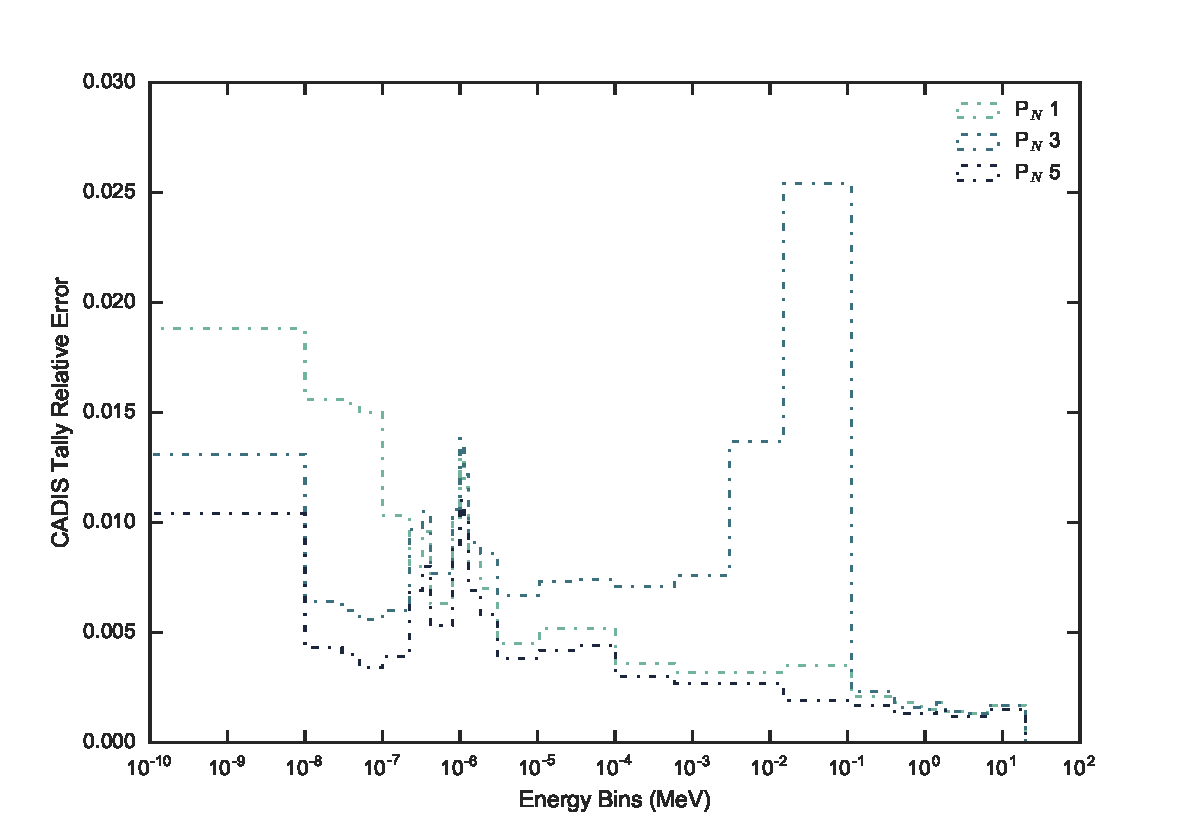
\includegraphics[width=\linewidth]{./chapters/characterization_probs/figures/angle/prob_1/err_pN_cadis.pdf}
    \caption{Relative errors of CADIS results for differing P$_N$ orders.}
    \label{fig:pn_cad_err}
  \end{subfigure}
\end{figure}
\begin{figure}[htb!]\ContinuedFloat
  \centering
  \begin{subfigure}[t]{\textwidth}
    \centering
    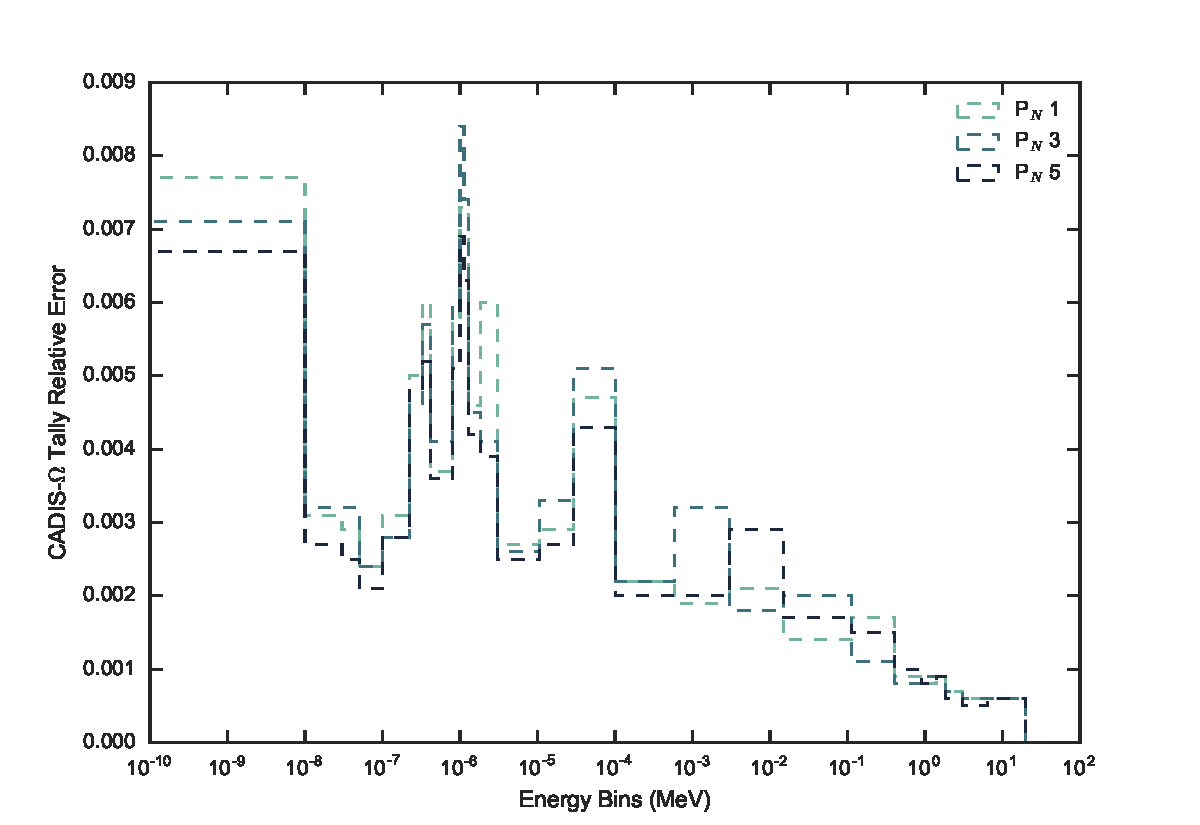
\includegraphics[width=\linewidth]{./chapters/characterization_probs/figures/angle/prob_1/err_pN_cadisangle.pdf}
    \caption{Relative errors of CADIS-$\Omega$ results for differing P$_N$
    orders.}
    \label{fig:pn_cadangle_err}
  \end{subfigure}
  \caption[Relative error results for CADIS and CADIS-$\Omega$ with changes in
  P$_N$ order for the problem with a steel beam in concrete.]
  {Relative error results for CADIS and CADIS-$\Omega$ with changes in
  P$_N$ order for the problem with a steel beam in concrete.}
  \label{fig:quad_errs}
\end{figure}

Figures \ref{fig:pn_cad_err} and \ref{fig:pn_cadangle_err} provide additional
information on interpreting Table \ref{tab:pn_foms}. Figure \ref{fig:pn_cad_err}
shows the tally relative error results for each of the P$_N$ order CADIS runs,
and Figure
\ref{fig:pn_cadangle_err} shows the relative error results
for CADIS-$\Omega$. In Figure
\ref{fig:pn_cad_err} the highest relative error for CADIS'
P$_N$ order 1 is the most thermal energy bin, for P$_N$ order 3 is the tally bin
between $10^{-2}$, and for P$_N$ order 5 is the resonance region around
$10^{-6}$. The lowest relative error bin, however, is the same for all P$_N$
orders. This bin is located just below the highest energy bin. The shifting
location of the highest valued relative error energy bin helps to explain the
strange trend of the FOMS in the second region of Table \ref{tab:pn_foms}.
Because the relative error bins  become larger in epithermal
energy groups at P$_N$ order 3, and this shift spans several energy bins, it
also helps to explain the tally average FOM shift to a lower value at P$_N$
order 3.

In Figure \ref{fig:pn_cadangle_err}, no significant shift in the relative error
happens at P$_N$ order 3. However, we can observe a shifting location of the highest
valued relative error. At P$_N$ order 1 the highest valued relative error for
CADIS-$\Omega$ is the lowest energy bin. At P$_N$ order 3 the highest relative
error bin is the resonance region located near $10^{6}$ MeV,  and at P$_N$ order
5 these two bins appear to have a similar relative error. The highest overall
observed relative error occurs in P$_N$ order 3, which is why we see the shift
to a lower FOM at P$_N$ order 3 for the maximum relative error subsection of
Table \ref{tab:pn_foms}. This shift is not as significant as the several-bin
spanning shift in CADIS, so it does not affect the tally average FOM in
CADIS-$\Omega$.

From Figures \ref{fig:pn_cadangle_err} and \ref{fig:pn_cad_err}, we can conclude
that shifts in the relative error that dramatically change between P$_N$ orders
can affect the overall tally convergence. This shift is not predictable, and may
not be observed if combined with a different set of deterministic parameters,
such as quadrature order 15, where both CADIS and CADIS-$\Omega$ have no spikes
in their relative errors.

\begin{figure}[h!]
  \centering
  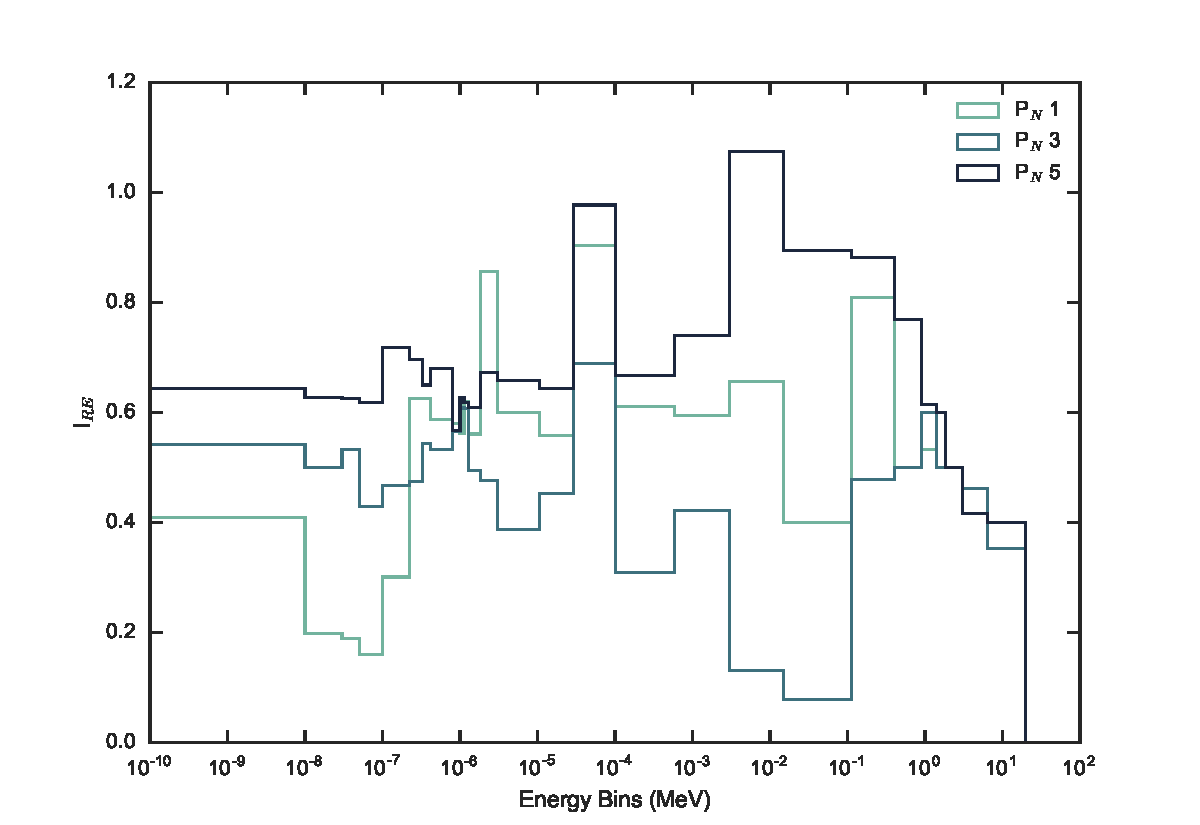
\includegraphics[height=10cm]{./chapters/characterization_probs/figures/angle/prob_1/compare_err_pN.pdf}
  \caption[Relative error improvement factor (Eq. \eqref{eq:I-RE}) between CADIS-$\Omega$ and
  CADIS with changes in P$_N$ order for steel beam embedded in concrete.]
  {Relative error improvement factor (Eq. \eqref{eq:I-RE}) between CADIS-$\Omega$ and
   CADIS with changes in P$_N$ order for the problem with a
   steel beam embedded in concrete.}
  \label{fig:prob_1_pN_I_RE}
\end{figure}

Figure \ref{fig:prob_1_pN_I_RE} shows the relative error improvement factor by
different P$_N$ orders. This plot complements what was observed in Figure
\ref{fig:prob_1_quad_I_RE}. Recall that a value below unity indicates that
CADIS-$\Omega$ achieved a better relative error than CADIS for a given energy
bin and quadrature order. First, with the exception of a few energy bins in
P$_N$ order 5, CADIS-$\Omega$ has better relative errors than CADIS for the
majority of P$_N$ orders and energy bins. In general, P$_N$ order 3 has the most
energy bins that obtain low values of I$_RE$, and P$_N$ order 5 has the fewest.

Another interesting feature
illustrated in this plot is that different P$_N$ orders perform the best in
distinct energy regions. At low energies P$_N$ order 1 achieves the best
relative errors, at intermediate energies P$_N$ order 3 achieves the best
relative errors, and at high energies all three perform similarly.

For all three
P$_N$ orders, the energy bin located near $10^{-4}$ MeV is problematic.
Returning again to the relative error plots of Figures \ref{fig:pn_cad_err}
and \ref{fig:pn_cadang_err}, this
particular energy bin had a spike for CADIS-$\Omega$, but remained relatively
small for CADIS. The consistency in each method's performance across all P$_N$
orders is reflected in this problematic energy bin.

\begin{figure}[h!]
  \centering
  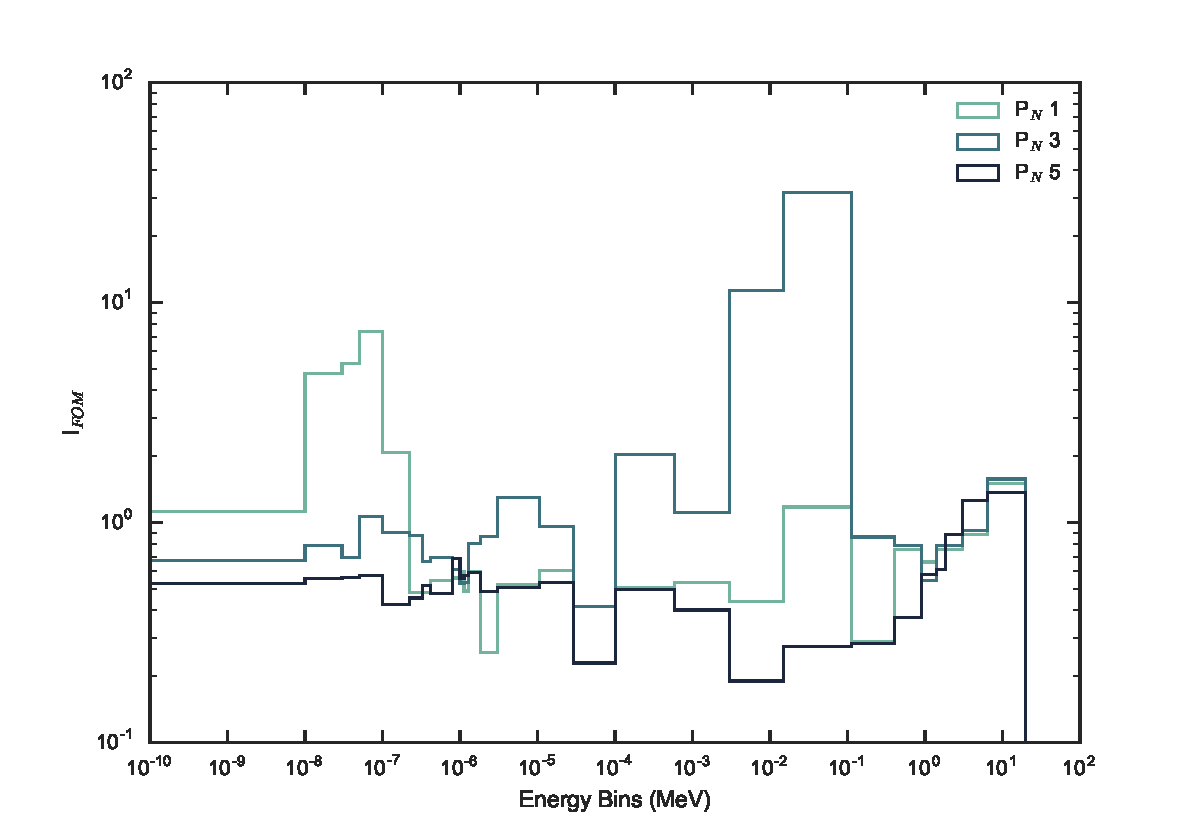
\includegraphics[height=10cm]{./chapters/characterization_probs/figures/angle/prob_1/compare_fom_pN.pdf}
  \caption[Figure of merit improvement factor (Eq. \eqref{eq:I-FOM}) between CADIS-$\Omega$ and
  CADIS as a function of P$_N$ order for steel beam embedded in concrete.]
  {Figure of merit improvement factor (Eq. \eqref{eq:I-FOM}) between CADIS-$\Omega$ and
   CADIS as a function of P$_N$ order for the problem with a
   steel beam embedded in concrete.}
  \label{fig:prob_1_pN_I_FOM}
\end{figure}

Figure \ref{fig:prob_1_pN_I_FOM} shows the FOM improvement factor with
increasing P$_N$ order. As with the quadrature orders, the runtimes of
CADIS-$\Omega$ impact the FOMs that it achieves such that many more energy bins
are more in CADIS' favor than in the relative error plot. However, many more
energy bins are above $10^0$ I$_{FOM}$ in P$_N$ order than for quadrature order.
As with I$_{RE}$, the shift in performance in different energy groups changes
with P$_N$ order. At low energies, P$_N$ order 1 achieves the best FOMs for
CADIS-$\Omega$, at intermediate energies P$_N$ order 3, and at high energies all
three P$_N$ orders have superior performance with CADIS-$\Omega$.

It should be
noted that there is no P$_N$ order for which CADIS-$\Omega$ obtains better FOMs
than CADIS in all energy bins. Contrast this to the relative error plot, where
CADIS-$\Omega$ had almost universally better relative errors than CADIS. Again
this undescores the negative impact that time has on CADIS-$\Omega$'s FOM.

% [Show FOMs as a function of pN order for first problem] \\
%
% [Show interesting anisotropy plots for extreme-valued pN orders] \\
%
% [Show flux maps for each extreme-valued problem in region of interest.] \\
%
% [Describe results.] \\
%
% [Show FOMs as a function of pN order for second problem] \\
%
% [Show interesting anisotropy plots for extreme-valued pN orders] \\
%
% [Show flux maps for each extreme-valued problem in region of interest.] \\
%
% [Describe results.] \\

\subsection{General Observations}
\label{subsec:observations}

At this point we are interested in which deterministic parameter value affects
CADIS-$\Omega$ and CADIS' performance more significantly. We
have looked at how varying each metric changes the relative error, I$_{RE}$, and
I$_{FOM}$, and from that we have observed trends associated with varying each
parameter. However, we have not compared each metric against the other.
Figures \ref{fig:angle_err_improvements} and \ref{fig:angle_fom_improvements}
aid in this comparison. As with P$_N$ order and S$_N$
order, these plots show either the relative error or Figure of Merit results for
the angle sensitivity study. Unlike the plots with I$_{RE}$ and I$_{FOM}$, these
figures show how the FOM and relative error change for a single method. That is,
how much does the relative error or the Figure of Merit change between the lowest-
and highest- valued parameters run for CADIS or CADIS-$\Omega$.
These figures are useful to show how
sensitive CADIS and CADIS-$\Omega$ are to P$_N$ order and quadrature order,
respectively.

In Figure
\ref{fig:angle_err_improvements}, the ratio of the relative error in each tally
bin is taken between the lowest and highest-valued parameter run of the
parametric study. For P$_N$ order (the purple lines in the figure)
this is calculated with $RE_{P_N 1}/RE_{P_N 5}$ and for
quadrature order (the green lines in the figure) it is calculated with
$RE_{S_N 5}/RE_{S_N 20}$.
A ratio above unity means that the relative error obtained by
the higher-valued parameter (P$_N$ order 5 or S$_N$ order 20) is lower than that
of the lower-valued parameter.

\begin{figure}[h!]
  \centering
  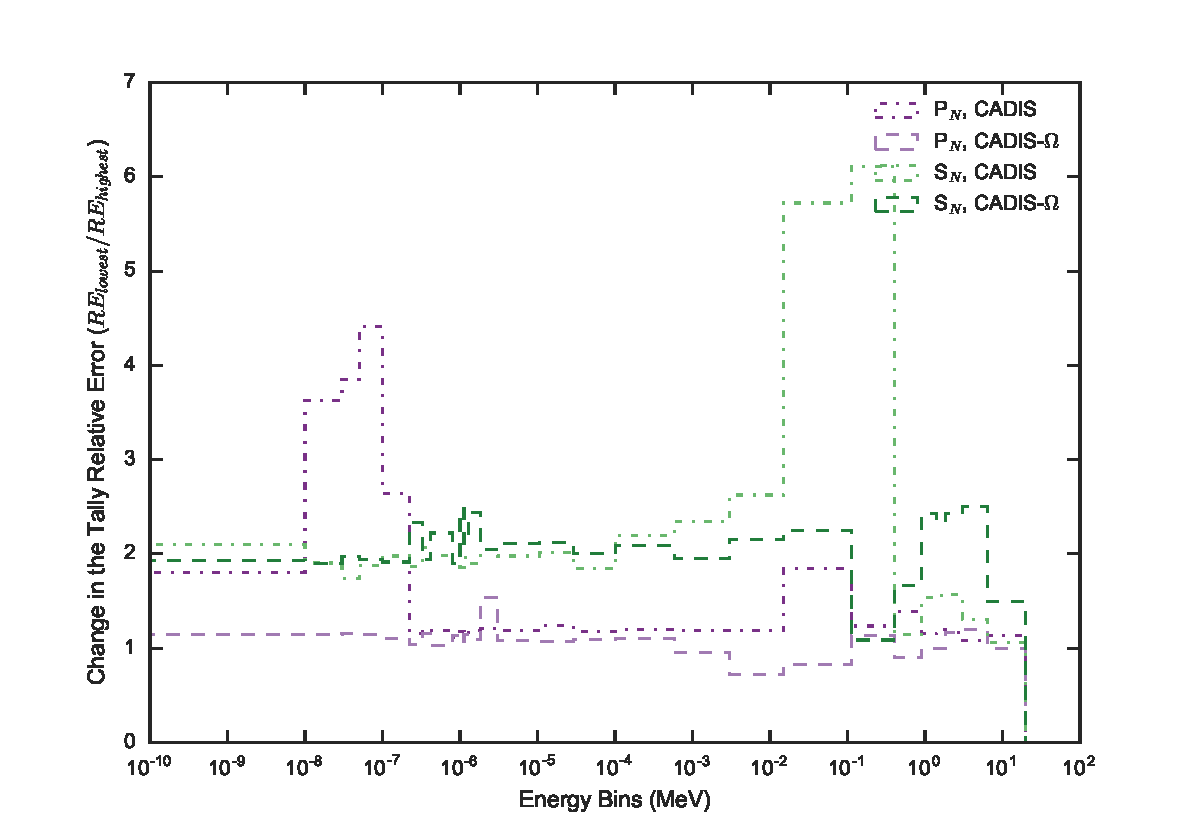
\includegraphics[height=10cm]{./chapters/characterization_probs/figures/angle/prob_1/improvement_err_allmethds.pdf}
  \caption[Ratio in the relative errors between the lowest and highest variable in the angle
  sensitivity study for CADIS and CADIS-$\Omega$.]{Ratio in the relative errors between
    the lowest and highest variable in the angle sensitivity study for CADIS and CADIS-$\Omega$.}
  \label{fig:angle_err_improvements}
\end{figure}

Figure \ref{fig:angle_err_improvements} shows that a greater change in the
relative error occurs for both CADIS and CADIS-$\Omega$ from S$_N$ order 5 to 20
than it does for P$_N$ orders. A notable exception to this is for CADIS in the
energy range from $10^{-8}$ to $10^{-7}$ MeV, where the relative error
improvement for P$_N$ order exceeds any quadrature order line.
Returning to
the relative error results for just CADIS, as shown in Figure
\ref{fig:pn_cad_err}, this energy range has a very high relative error for P$_N$
order 1, especially when compared to the other energy regions nearby. In this
energy range, the relative error drops from 0.015 to .005 from P$_N$ order 1 to
3, but the energy bin immediately adjacent
only drops about .005 total. The greater change
in the relative error for this region accounts for the spike we see in Figure
\ref{fig:angle_err_improvements}.

The data in this figure also shows us that increasing P$_N$ order for
CADIS-$\Omega$ does not reduce the relative error in the energy range from
$10^{-3}$ to $10^{0}$ MeV. CADIS-$\Omega$'s purple line on this figure is
located below unity in that energy region. Generally this line for
CADIS-$\Omega$ does not see a huge improvement with increasing P$_N$ order.
For a problem like this, a low P$_N$ order may be a good enough choice.

CADIS' results in the same energy region show improvement in the
relative error. However, in many centrally-located energy bins, this improvement
is very small. If a tally existed for a similar problem in these energy ranges,
it may be sufficient to use CADIS with a low P$_N$ order as well.

\begin{figure}[h!]
  \centering
  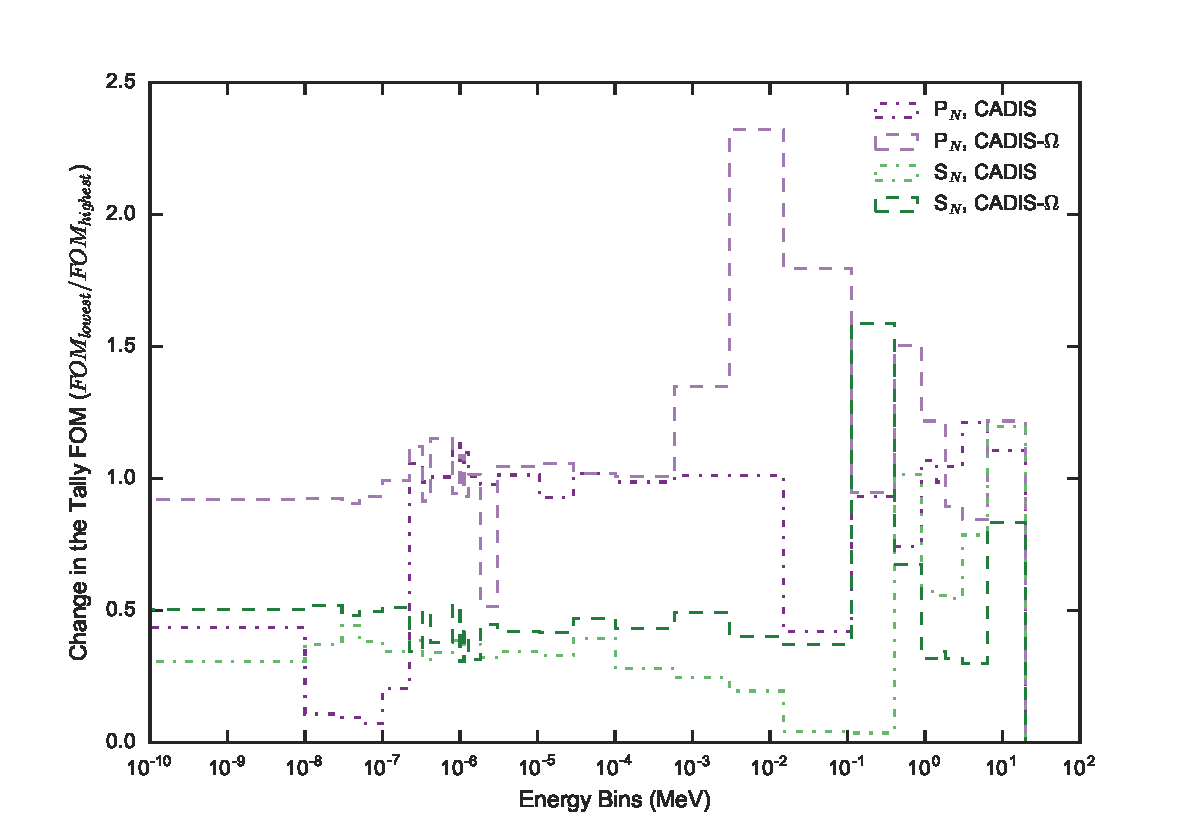
\includegraphics[height=10cm]{./chapters/characterization_probs/figures/angle/prob_1/improvement_fom_allmethds.pdf}
  \caption[Ratio in the figure of merits between the lowest and highest variable in the angle
  sensitivity study for CADIS and CADIS-$\Omega$.]{Ratio in the figure of merits between
    the lowest and highest variable in the angle sensitivity study for CADIS and CADIS-$\Omega$.}
  \label{fig:angle_fom_improvements}
\end{figure}

In Figure \ref{fig:angle_fom_improvements}, the linestyles and colors match
those in Figure \ref{fig:angle_err_improvements}. The y-axis of this figure
shows the ratio of the FOMs for the lowest- and highest-valued parameters. The
purple lines are calculated by the ratio of $FOM_{P_N 1}/FOM_{P_N 5}$;
the green lines show the
ratio of $FOM_{S_N 5}/FOM_{S_N 20}$; the linestyles indicate the method
type. In this plot, a low-valued ratio reflects a higher valued FOM obtained by
the finer P$_N$ or S$_N$ order.

Some features from \ref{fig:angle_err_improvements} are continued in Figure
\ref{fig:angle_fom_improvements}. For example, the energy bins between $10^{-8}$
and $10^{-7}$ MeV still show a large change for P$_N$ order in CADIS. However,
the addition of time to calculate the FOMs affects both methods. In Figure
\ref{fig:angle_err_improvements}, we observed that for both methods, increasing
P$_N$ order or quadrature order generally decreased the relative error. In
Figure \ref{fig:angle_fom_improvements}, this is not the case. At low energies,
all methods have higher FOMs with increasing parameter resolution. At
intermediate energies, only S$_N$ order strongly changes the FOM. At high
energies, energy bins for both S$_N$ and P$_N$ order wildly oscillate between
improved and not improved.

The CADIS lines in Figure \ref{fig:angle_fom_improvements} generally lie at
lower values than CADIS-$\Omega$. Consequently, larger changes in the FOM are
observable with increasing either P$_N$ or S$_N$ order. This is the case for
most energy bins, but not above $10^0$ MeV. In this region, CADIS-$\Omega$ and
CADIS shift between energy bins in which method sees
a larger change with parameter value selection.

By inspecting both Figure \ref{fig:angle_err_improvements} and
\ref{fig:angle_fom_improvements}, a few common themes appear. First, CADIS has a
larger change in the tally relative error and FOM than CADIS-$\Omega$ for most
energy bins. Second, this general observation does not hold for energy bins
greater than $~10^{-1}$. At these energy regions, CADIS-$\Omega$ achieves a
better relative error with increasing S$_N$ order, but not P$_N$ order. Neither
CADIS-$\Omega$ or CADIS have a dominant trend in FOM values in this region.
Another observation is that generally S$_N$ order has a greater effect on the
relative errors and FOMS for both methods. This is not the case in the high
energy region for FOM values, where both methods are comparable.

